\section{Experiments}
\label{experiments}

a) \emph{Debugging the pacemaker}: As an illustration of how a Virtual Heart Model (VHM) can be used to debug a pacemaker, we give a simple example of a pacemaker model in Simulink, connected to a VHM in Simulink as well. 
The pacemaker and VHM models are shown in Fig.~\ref{fig:simulinkModels}.
\begin{figure}[tb]
	\centering
	
\includegraphics[scale=0.2]{placeHolder.pdf}
	\caption{Simulink models of heart and pacemaker.}
	\label{fig:simulinkModels}
\end{figure}
No open-loop testing was conducted on the pacemaker model.
However, 
The requirement given to the tester was that if a PVC or $V_{sense}$ or $V_{pace}$ occur, then the next $V_{pace}$ should not occur before 500ms. 
\todo[inline]{ZJ : why is this a requirement of good behavior?}
The specification-guided testing methodology outlined in Section \ref{closedloop} quickly found a PVC disturbance waveform that caused the closed loop to violate this specification (fewer than 10 tests).
Debugging revealed that the pacemaker model was missing the behavior that caused it to reset the Upper Rate Interval to its default value after every VS event.

For the next two experiments, we used a pacemaker model that had been open-loop tested to satisfy a number of specifications from the Boston Scientific Challenge \cite{challenge}.
\todo[inline]{ZJ, RM: is this last stmt true?}

b) \emph{Exploring behavior}: In this experiment, we set a minimum delay of 400ms between PVC pulses, and tried to falsify the following specification:
``If either Node3 depolarizes because of path conduction or a VP is issued, a minimum of 500ms must pass before the next VP".
\todo[inline]{ZJ :why is this a requirement of good behavior?s}
Note that the pacemaker can not distinguish between a VS caused by a PVC and a VS caused by path conduction.
\todo[inline]{ZJ : cite}
Thus we need access to the heart model to test this specification, and this can only happen in a closed-loop setting.

The specification was violated by the waveform shown in Fig. \ref{fig:bug8_kept1}.
\begin{figure}[tb]
\centering
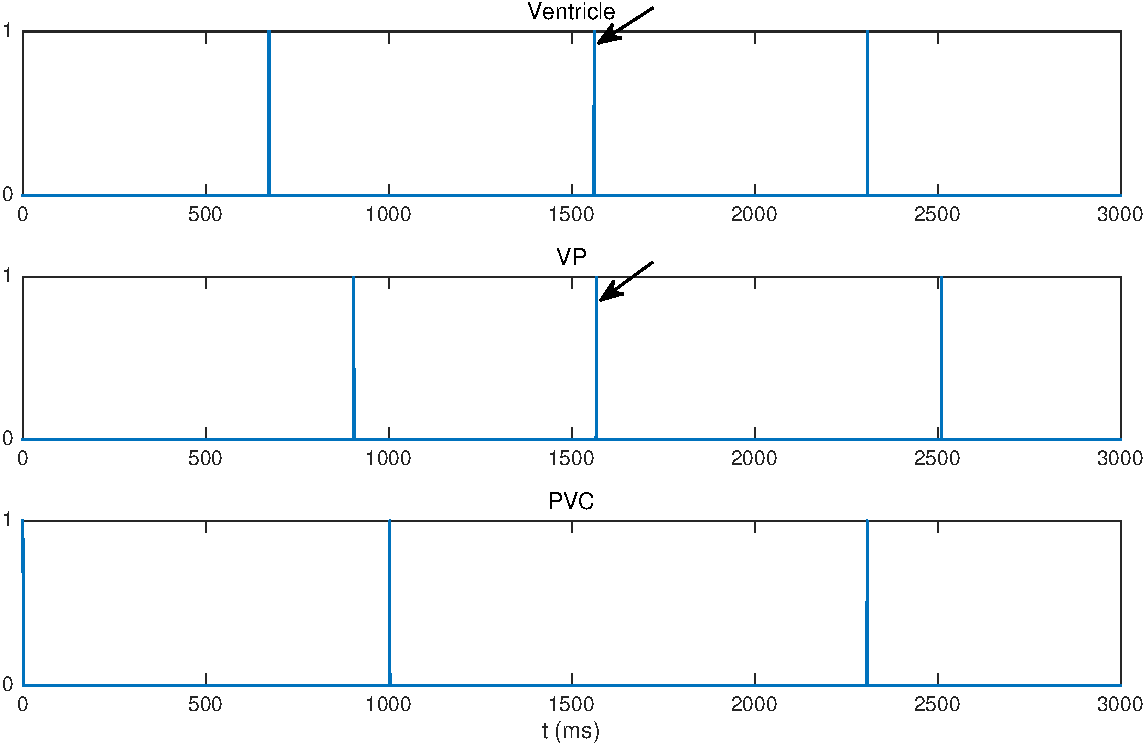
\includegraphics[width=0.7\linewidth]{figures/bug8_kept1}
\caption{A PVC pattern that causes a premature ventricular pacing.}
\label{fig:bug8_kept1}
\end{figure}
Upon investigating the reasons for this violation, it was concluded that the Ventricular Safety Pacing (VSP) feature of our model was at fault: the VSP is a way to prevent the consequences of AV crosstalk, namely, self-inhibition. 
When the pacemaker senses a ventricular event during the VSP interval (but past the PAVB interval), it schedules a $V_{pace}$ to be executed at the end of the VSP.
In this experiment, a PVC disturbance that occurred past the PAVB, but still within the VSP, provoked the ventricular event that led to the early VP.

In this case, the violating trace is due to a desired feature of the pacemaker (preventing self-inhibition).
Thus, the designer and physician must decide whether this is an acceptable case, or the pacemaker needs to be adjusted (if at all possible) to prevent this from happening (while maintaining the VSP safety feature).

c) \emph{Finding harmful heart behavior}: In this experiment, we tested the closed loop to see if the pacemaker could lead the heart into a harmful condition known as Endless Loop Tachycardia (ELT).
%
The heart has one intrinsic conduction pathway from atria to ventricles, namely from the SA node to the ventricles via the AV node and His bundle.
The DDD pacemaker introduces another, virtual, pathway between the atrial lead and the ventricular lead.
Together, these form a closed circuit which can cause the heart to beat incessantly at a fixed high rate.
Specifically, if a PVC event is sensed by the pacemaker, it triggers V-A conduction along the intrinsic pathway, 
which in turn triggers Atrial Sense (AS). 
The pacemaker will then pace the ventricle (issue a VP) after TAVI ms according to its A-V synchrony function. 
This VP acts as the catalyst for another V-A conduction, and so on.
The conduction loop is then formed and the VP-AS pattern will persist if no actions are taken.
The heart rate is kept as high as the upper rate limit of the pacemaker since the cycle length of the conduction loop is very short. 
ELT is a harmful condition since a fast fixed heart rate that will cause inefficient pumping of blood.
Thus even though the pacemaker is correct according to its specification, it can still lead the heart into ELT if a PVC interferes with its operation as described.
%

S-Taliro was given the ELT specification, and a PVC constraint of at most 2 PVCs in a 10,000ms interval. 
The total test duration was $T= 10,000$ms.
S-Taliro found a PVC pattern, shown in Fig.\ref{fig:bug13_kept1}, that caused ELT.
\begin{figure}[t]
\centering
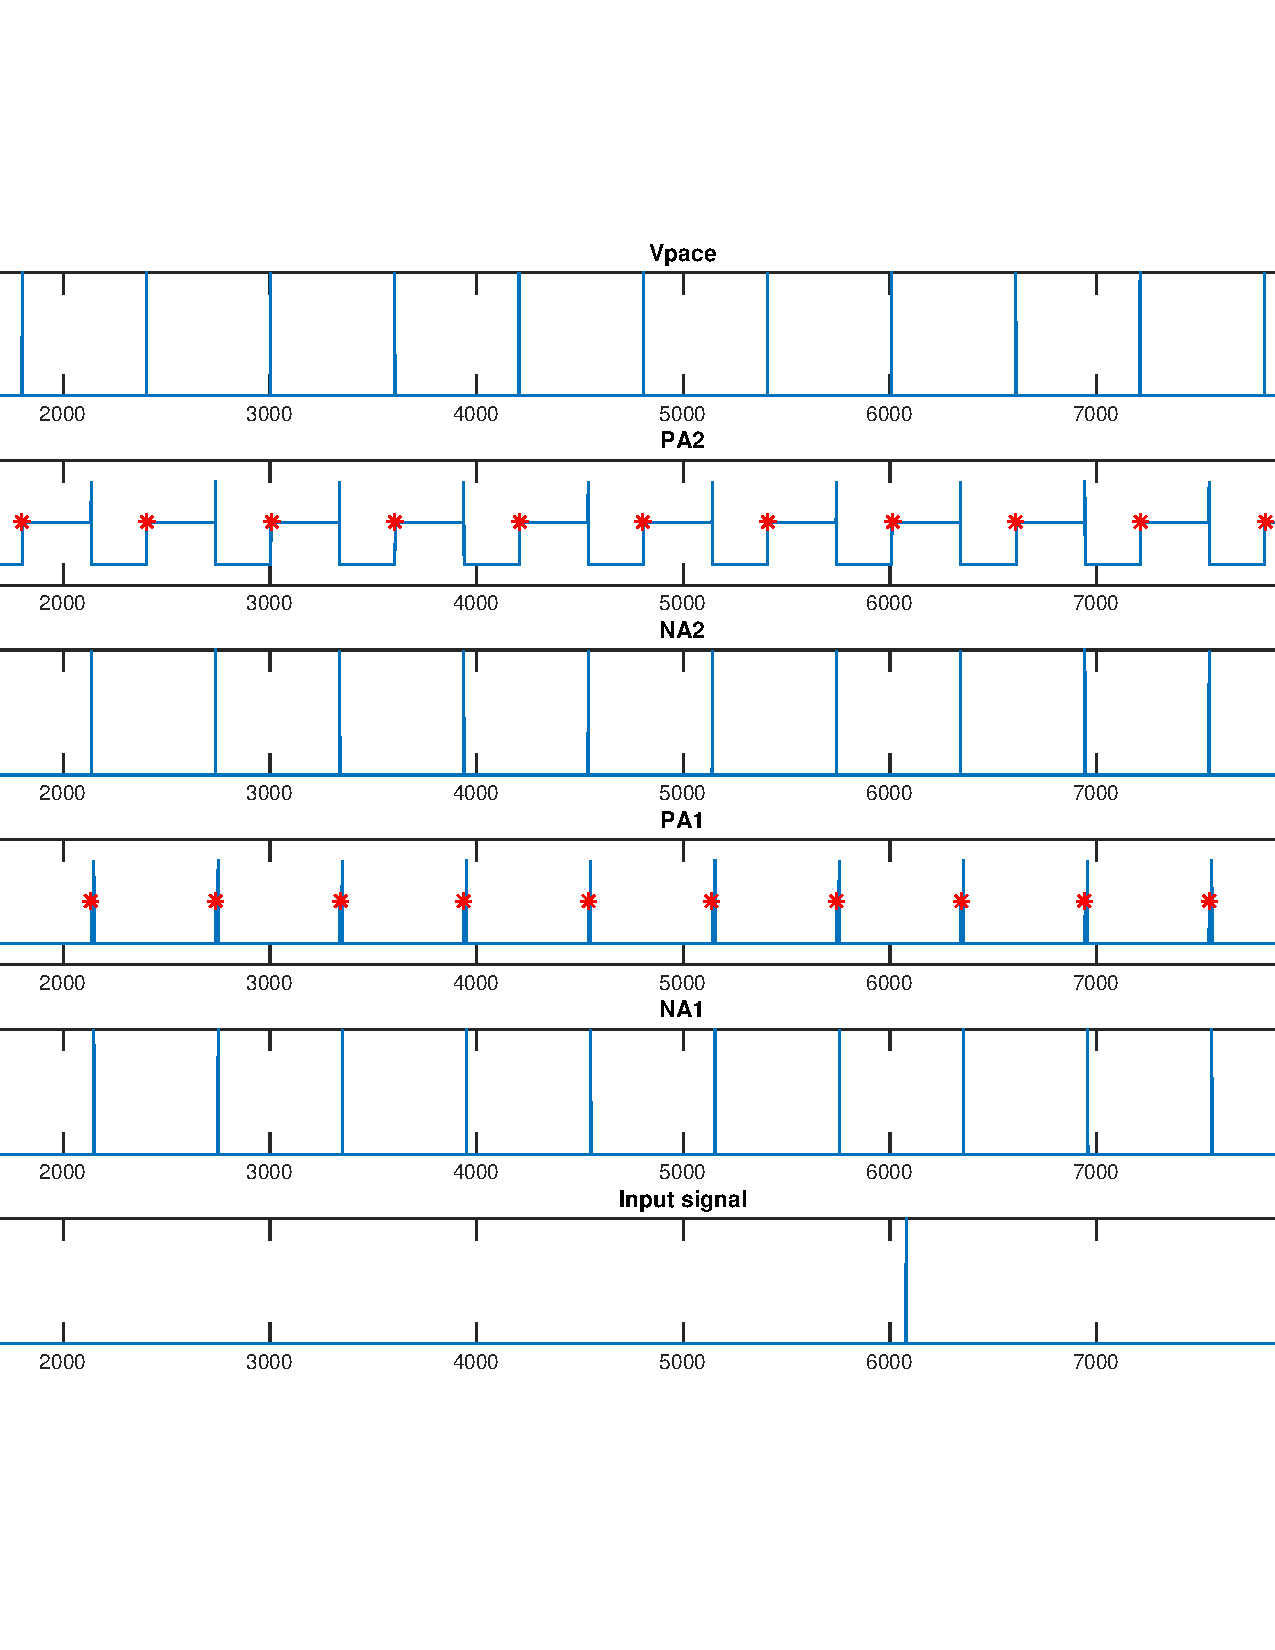
\includegraphics[scale=0.4]{figures/bug13_kept1}
\caption{ELT: successive cycles of VP induced by an initial PVC. Red stars indicate timing of backward path conduction.}
\label{fig:bug13_kept1}
\end{figure}


